% 6.344 (Digital Image Processing) Final Project
% Author: Michael Mekonnen

\documentclass[12pt]{amsart}

% Packages
\usepackage{hyperref}
\usepackage[pdftex]{graphicx}

% Custom commands
\newcommand{\HRule}{\rule{\linewidth}{0.5mm}}

\title{Edge Detection}

\begin{document}

\begin{titlepage}
\begin{center}

\textsc{\LARGE Massachusetts Institute of Technology}\\[1.5cm]

\textsc{\Large Digital Image Processing (6.344) \\ Final Project}\\[0.5cm]

\HRule \\[0.4cm]
{ \huge \bfseries Edge Detection}\\[0.4cm]
\HRule \\[1.5cm]

\large Michael \textsc{Mekonnen}

\vfill

{\large \today}

\end{center}
\end{titlepage}

\maketitle

\section{Introduction}

For my 6.344 final project, I took up the task of edge detection: given an image, produce a new image that clearly outlines the edges in the original image. This is a well studied idea, and there are various methods available. Here, I will explore two of the most widely used methods: the gradient-based method and the laplacian-based method.

\section{Gradient-based method}

The gradient-based method detects edges in a $2D$ image by finding the analogue of a gradient for the image and then finding the peaks of the magnitude of the gradient. It helps to think about this in $1D$. To find the ``edges" of a $1D$ continuous signal $f(x)$, we would first take the derivative $\frac{df}{dx}$ and look for it's optima since an edge in $1D$ is a fast change in $f(x)$ for a small change in $x$, which is we can very clearly detect by taking the derivative. For a $2D$ continuous signal $f(x,y)$, we can do a very similar thing. Here, we would find the magnitude of the gradient given by $|\nabla f(x,y)| = \sqrt{(\frac{\partial f}{\partial x})^2 + (\frac{\partial f}{\partial y})^2}$ and search for its optima. When we are working a digital image, we are not able to take derivatives, so we approximate the derivatives. There are various ways to approximate the derivatives $\frac{\partial f}{\partial x}$ and $\frac{\partial f}{\partial y}$, but one intuitive and standard method is to use filters like the ones shown in Figure TODO.

In Figure TODO, I present my overall gradient-based edge detection system. Given an image $f(n_1, n_2)$, we first finds its derivatives in the $n_1$ and $n_2$ directions exactly by using the filters shown in Figure TODO. Next, we compute an approximation of the magnitude of the gradient by taking the square root of the sum of the squares of the two different derivatives. The standard gradient-based edge detection method then proceeds to finding the pixels whose gradient magnitude exceeds some threshold, and these pixels are classified as edge pixels. This steps is usually followed by an edge-thinning step. The choice of this threshold depends on the particular image at hand. In my project, I chose to do something different from using an experimentally found threshold. I first find the maximum gradient magnitude, $M$. Then, for a given pixel $(n_1, n_2)$, I set its brightness level in the output image to be:
\begin{equation*}
255 \left(1 - \left(\frac{|\nabla f(n_1, n_2)|}{M}\right)^\alpha\right).
\end{equation*}
What this does is assign pixels whose gradient magnitude is close to $M$ a low brightness (close to $0$ or black) and assign pixels whose gradient magnitude is close to $0$ a hight brightness (close to $255$ or white). $\alpha$ is simply a tuning parameter. The resulting edge map traces the edges in the image, and highlights the more drastic edges more strongly. One important benefit of this method is that it avoids having to manually pick a threshold value for each image of interest. There is still the task of choosing the right value of $\alpha$, but I have observed from experimentation that the same value of $\alpha$ has a uniform effect over different images, so one may choose some default value of $\alpha$, for example $1$, and still obtain a reasonable result.

\begin{figure}
\begin{minipage}[b]{0.45\linewidth}
\centering
\begin{tabular}{c || c | c | c }
1 & -1 & 0 & 1 \\
\hline
0 & -1 & 0 & 1 \\
\hline
-1 & -1 & 0 & 1 \\
\hline\hline
& -1 & 0 & 1 \\
\end{tabular}
\end{minipage}
\hspace{0.5cm}
\begin{minipage}[b]{0.45\linewidth}
\centering
\begin{tabular}{c || c | c | c }
1 & 1 & 1 & 1 \\
\hline
0 & 0 & 0 & 0 \\
\hline
-1 & -1 & -1 & -1 \\
\hline\hline
& -1 & 0 & 1 \\
\end{tabular}
\end{minipage}
\caption{TODO}
\label{fig:TODO}
\end{figure}

\begin{figure}
\centering
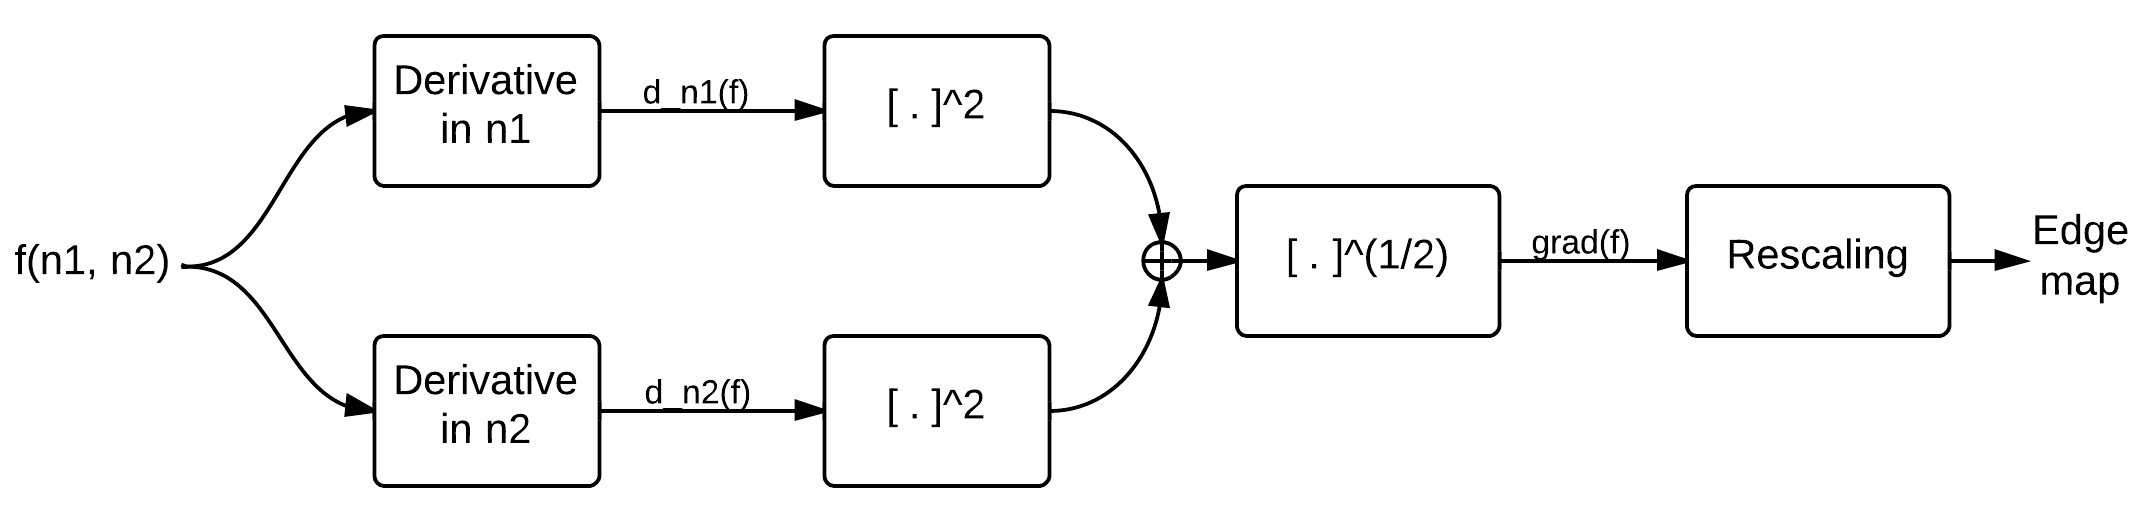
\includegraphics[width=\linewidth]{GradientMethod.png}
\caption{TODO}
\label{fig:TODO}
\end{figure}

\section{Laplacian-based method}

\begin{figure}
\centering
\begin{tabular}{c || c | c | c }
1 & -1 & 2 & -1 \\
\hline
0 & 2 & -4 & 2 \\
\hline
-1 & -1 & 2 & -1 \\
\hline\hline
& -1 & 0 & 1 \\
\end{tabular}
\caption{TODO}
\label{fig:TODO}
\end{figure}

\end{document}
